\documentclass[11pt]{beamer}
\usepackage[utf8]{inputenc}
\usepackage[T1]{fontenc}
\usepackage{lmodern}
\usetheme{CambridgeUS}
\usepackage{graphicx} 
\usepackage{verbatim}
\usepackage{xcolor} % For color customization

\begin{document}
	\titlegraphic{
\includegraphics[width=2.0cm]{/home/quentinb/PhdWork/3PG_Lec/UGAlogo.png}} % Ensure the correct path and file extension
	\setbeamerfont{title}{size=\large}
	\setbeamerfont{subtitle}{size=\small}
	\setbeamerfont{author}{size=\small}
	\setbeamerfont{date}{size=\footnotesize}
	\setbeamerfont{institute}{size=\footnotesize}
	\title[3PG: The Basics]{3PG: The Basics}%title
	%\subtitle{ }%%subtitle
	\author[Quentin Boccaleri]{Quentin Boccaleri\inst{1}}%%authors
	
	\institute[UGA]{The University of Georgia\inst{1}}
	\date[\textcolor{white}{Precision Silviculture, 2025}]
	{Precision Silviculture\\
		Aug XX, 2025}
		
	\AtBeginSection[]{
		\begin{frame}
			\centering
			\insertsectionhead
			\setbeamerfont{title}{size=\large}
		\end{frame}
	}
	
	
	\begin{frame}
		\titlepage
	\end{frame}


\begin{frame}
	\frametitle{Outline}
	\tableofcontents
\end{frame}

%------------------------------------------------------------
\section{What is 3PG?}

\begin{frame}
	\frametitle{The Big Picture}
	\begin{center}
		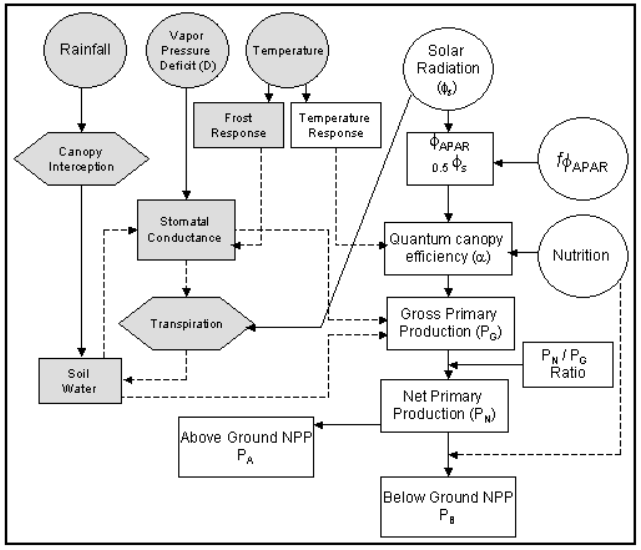
\includegraphics[width=8.0cm]{/home/quentinb/PhdWork/3PG_Lec/3PG.png.png}
	\end{center}
\end{frame}

\begin{frame}
	\frametitle{The Big Picture}
	\begin{center}
		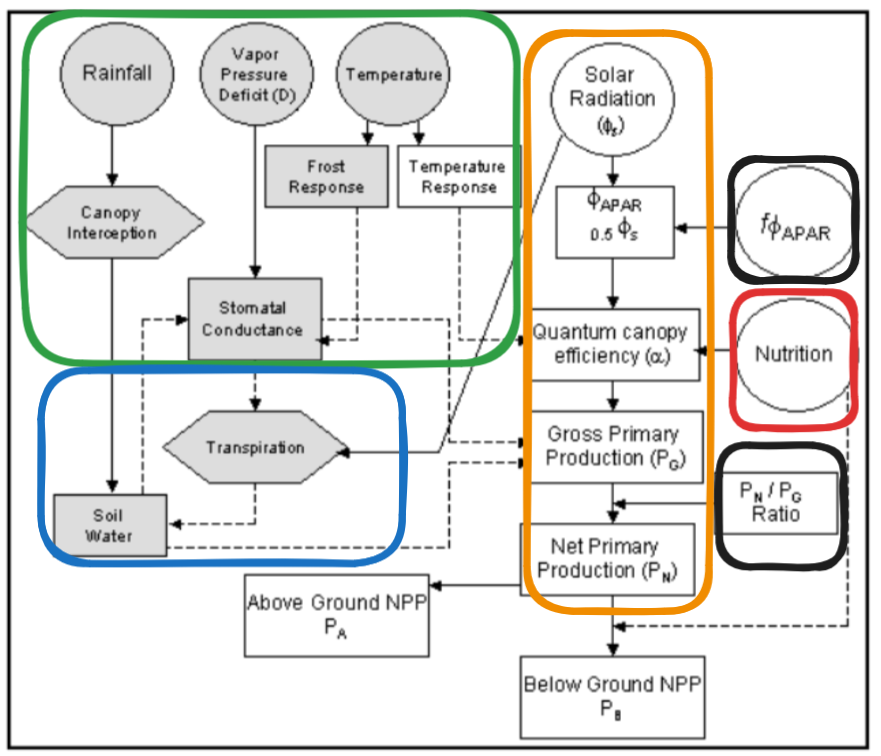
\includegraphics[width=8.0cm]{/home/quentinb/PhdWork/3PG_Lec/3PG2.png}
	\end{center}
\end{frame}

\section{The Engine of 3PG} 
\begin{frame}
	\begin{enumerate}
		\item 3PG begins with taking \textbf{incoming solar radiation}, and converting it into \textbf{Photosynthetically Active Radiation (PAR)}.
		\begin{center}
			$PAR = 0.5(GR)$
		\end{center}
		\begin{center}
			\textit{Where PAR and GR are in MJ per m per day.}
		\end{center}
		\vspace{3mm}
		\item PAR must then be converted into \textbf{GPP}.
		\begin{center}
			$P_g = \alpha_c(1-e^{-kL})Q_0$
		\end{center}
		\begin{center}
			\textit{Where $P_g$ is GPP (MJ per m per day), $\alpha_c$ is canopy quantum efficiency, $(1-e^{-kL})Q_0$ is Beer's Law.}
		\end{center}
		\vspace{3mm}
		\item GPP is then converted into \textbf{NPP} using a constant fraction of 0.47.
	\end{enumerate}
\end{frame}

\begin{frame}{r3PG}
	\begin{enumerate}
	\item An R package developed by Volodymyr Trotsiuk et al. based on code from Peter Sands Excel extension of 3PG and 3PG-mix. 
	\item Can do stand level and spatial level simulations. 
	\item Highly complex in terms of data preparation and formatting. Highly data frame dependent.
	\end{enumerate}  
\end{frame}



\begin{frame}
	\frametitle{R Code Example}
		\begin{verbatim}
		library(r3PG)
		out_3PG <- run_3PG(
		site        = d_site, 
		species     = d_species, 
		climate     = d_climate, 
		thinning    = d_thinning,
		parameters  = d_parameters, 
		size_dist   = d_sizeDist,
		settings    = list(light_model = 2, transp_model = 2, phys_model = 2, 
		height_model = 1, correct_bias = 0, calculate_d13c = 0),
		check_input = TRUE, df_out = TRUE)
		
		head(out_3PG)
		\end{verbatim}
\end{frame}


\end{document}
